\documentclass{article}
\usepackage{CJK}
\usepackage{amsmath}
\usepackage{amsthm}
\usepackage{amsfonts}
\usepackage{palatino}
\usepackage{xcolor}
\usepackage{geometry}
\usepackage{listings}
\usepackage{pxfonts}
\usepackage{enumerate}
\usepackage[pdftex]{graphicx}
\geometry{left=2cm,right=2cm,top=3cm,bottom=3cm}
\pagestyle{myheadings}
\markright{Huiqian Yu/14300180118}
\setlength{\parindent}{0pt}
\newcommand{\ix}[1]{\intertext{{}#1}}
\newcommand{\dx}{\;\mathrm{d}\,x}
\newcommand{\dt}{\;\mathrm{d}\,t}
\newcommand{\dm}[1]{\;\mathrm{d}\,{}#1}
\newcommand{\ve}{\varepsilon}
\newcommand{\tp}{^\mathsf{T}}
\newcommand{\var}{\mathrm{var}}
\newcommand{\corr}{\mathrm{corr}}
\newcommand{\mbe}[1]{\mathbb{E}\left[{}#1\right]}
\begin{document}

\definecolor{backcolour}{rgb}{0.95,0.95,0.92}
\begin{CJK*}{GBK}{song}
\begin{enumerate}
\section{Homework03}
\item[3.1]
\begin{align*}
    \rho _x(1)&=\dfrac{\gamma (x_t,x_{t-1})}{\gamma (0)}\\
    &= \dfrac{\mbe{x_tx_{t-1}}}{\mathrm{var}(w_t+\theta w_{t-1})}\\
    &= \dfrac{\theta \sigma_w^2}{(1+\theta^2)\sigma_w^2}\\
    &= \dfrac{\theta}{1+\theta^2}\\
    |\rho_x(1)|&= \dfrac{|\theta|}{1+\theta^2}\\
\ix{The equality holds if and only if}
    |\theta|&=1
\end{align*}
That is, for $\theta=-1$, $\rho_x(1)$ attains its minimum $-\dfrac{1}{2}$; for $\theta=1$, $\rho_x(1)$ attains its maximum $\dfrac{1}{2}$.
\begin{center}
%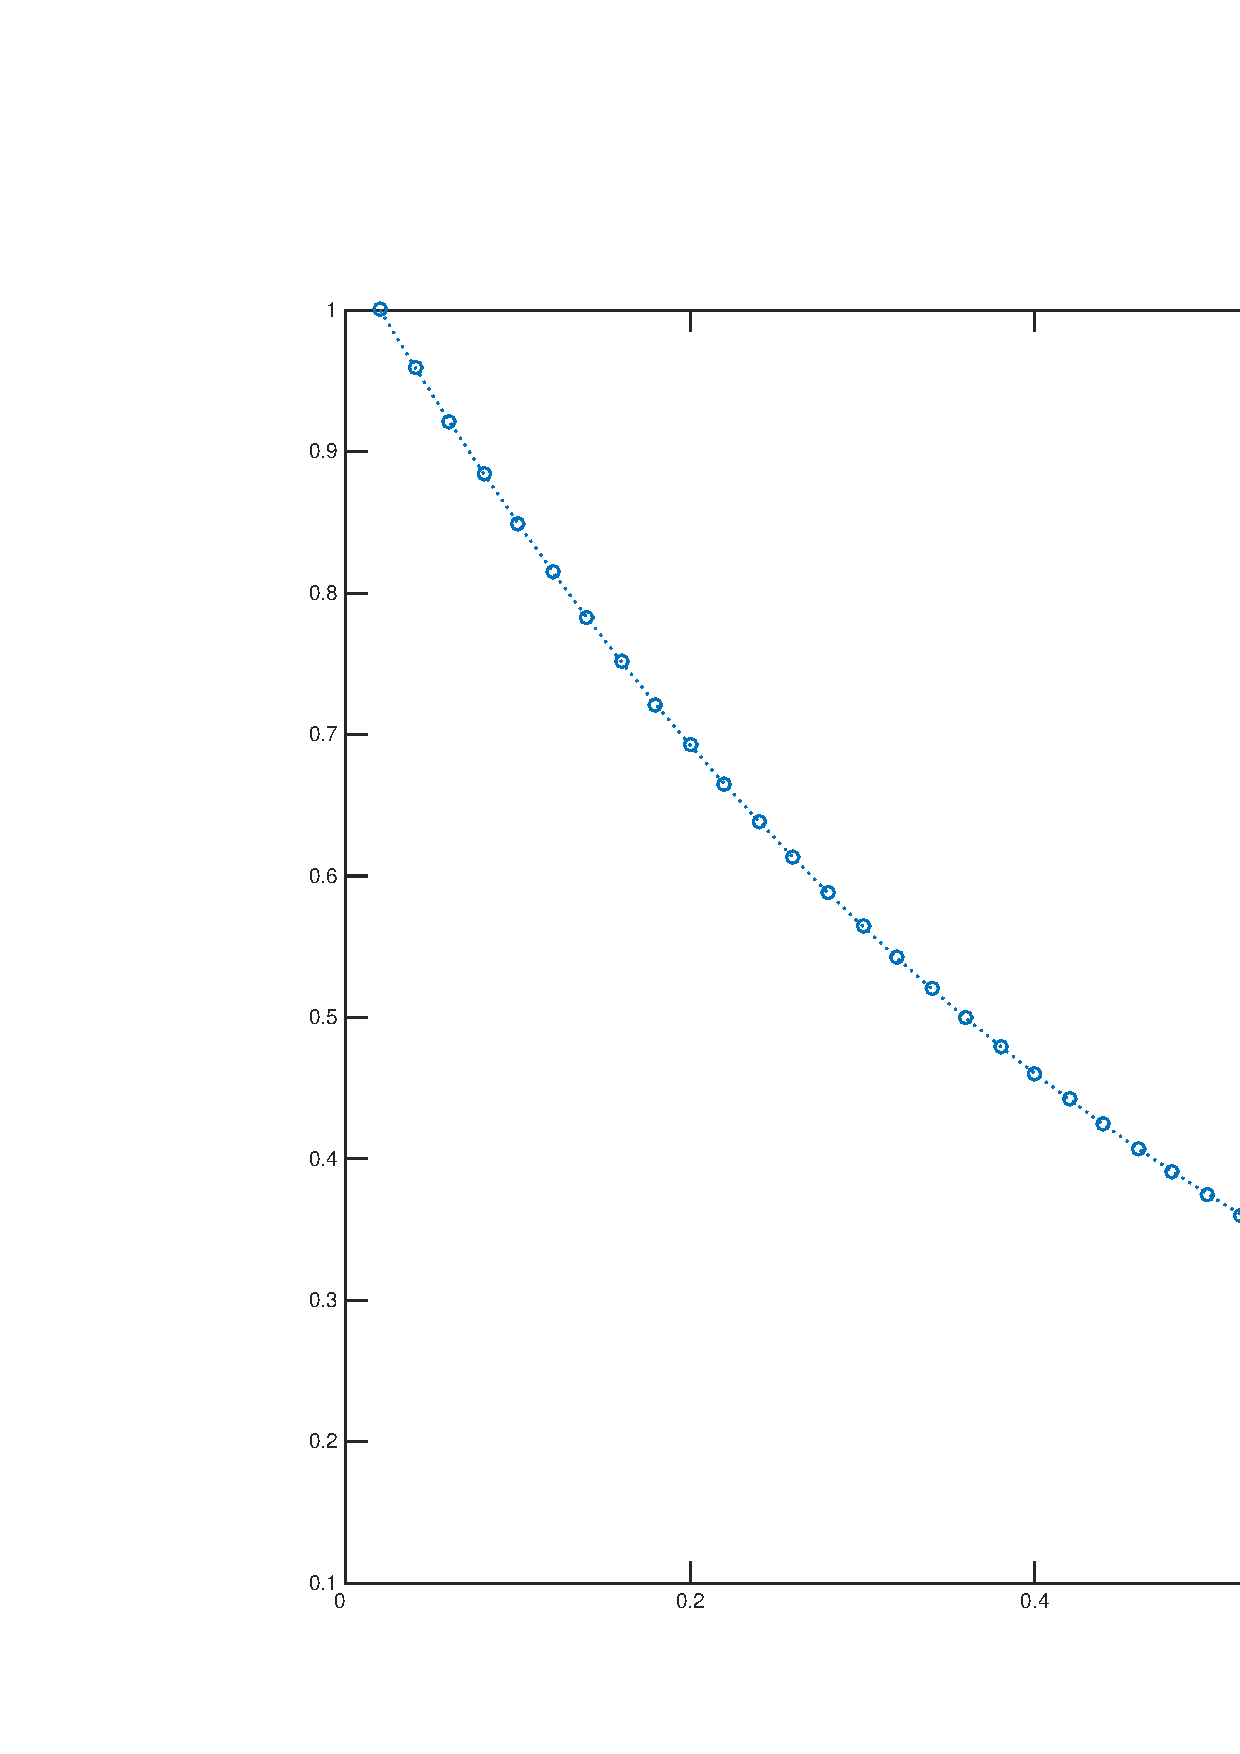
\includegraphics[width=8cm]{1.png}
%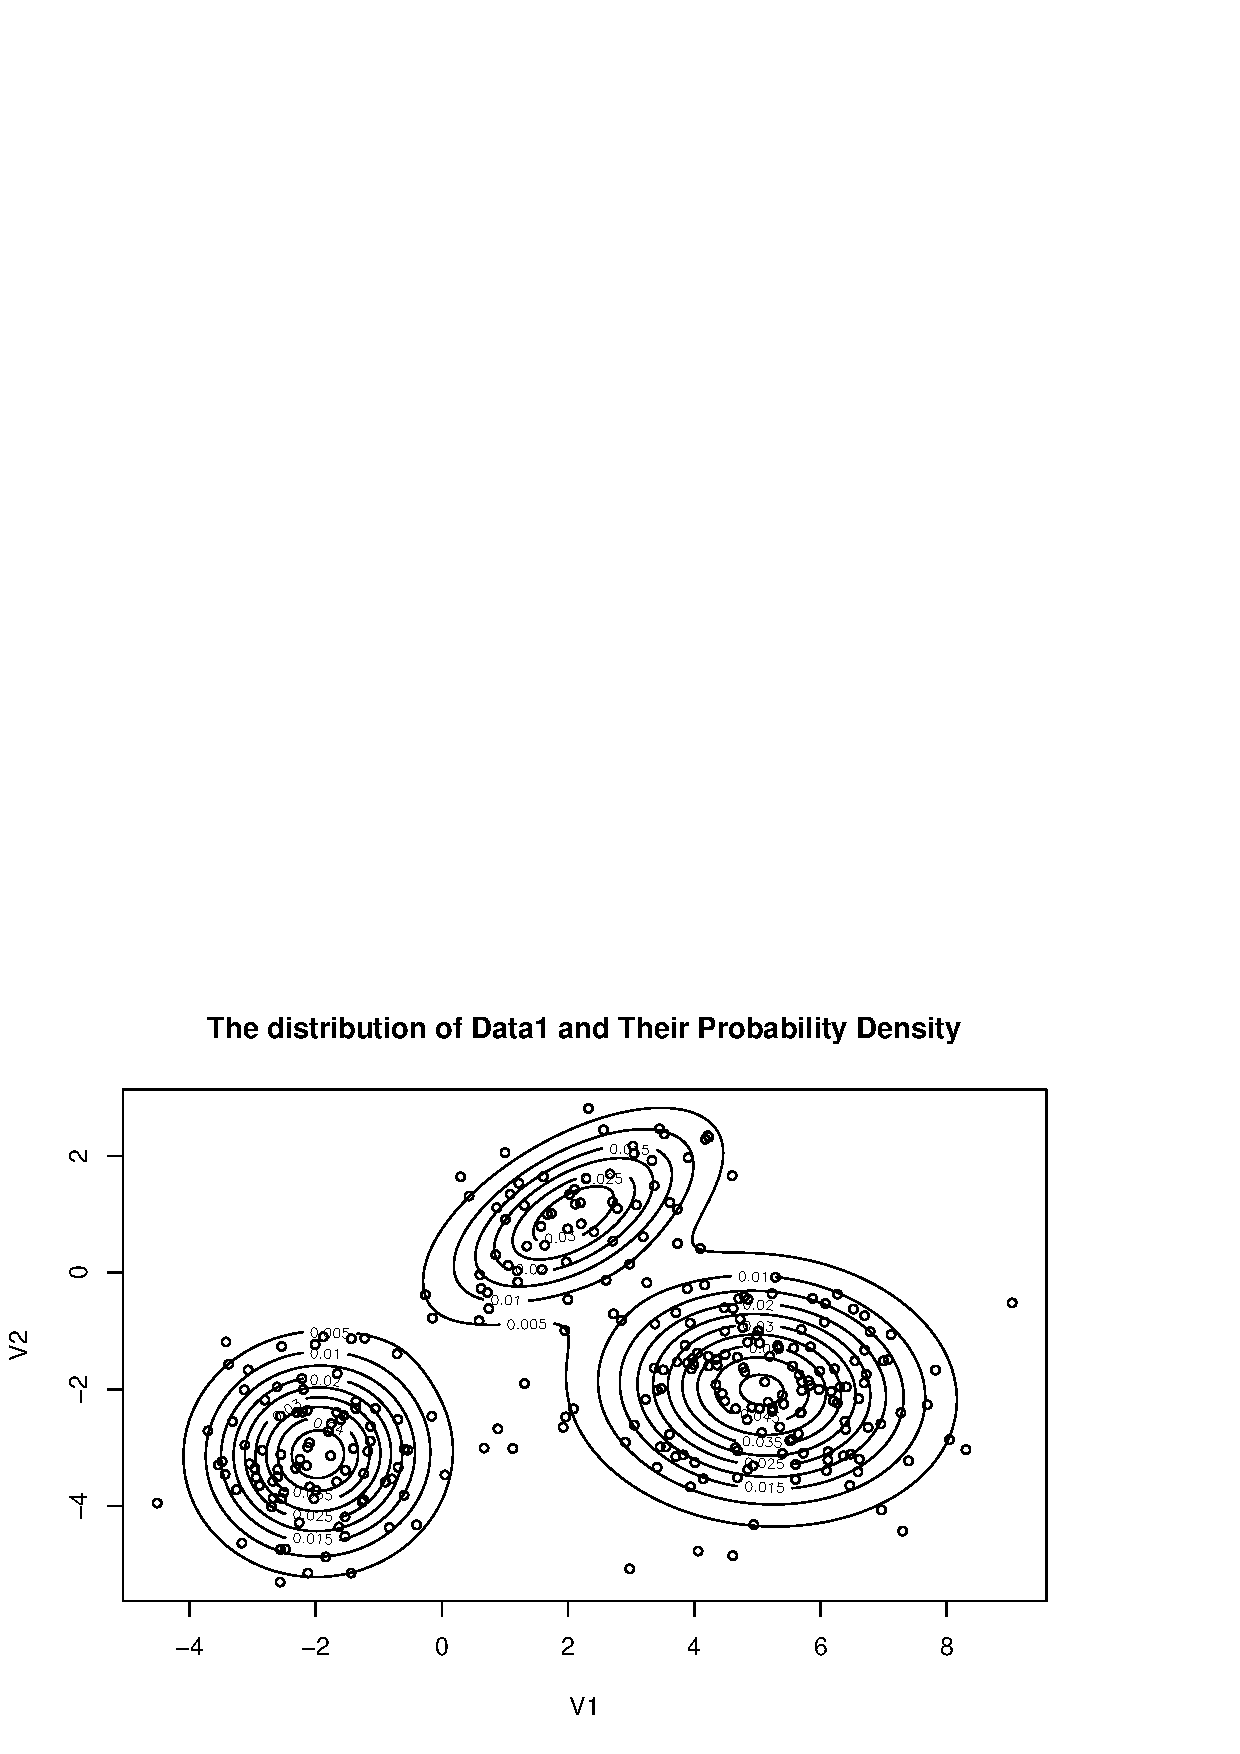
\includegraphics[width=8cm]{2.png}
\end{center}
\item[3.2]
\begin{align*}
\ix{(a)}
    x_t&=   \sum\limits_{i=0}^{t-1} \phi^iw_{t-i}\\
    \mu_x(t)&=0\\
    \var _x(t)&= \sum\limits_{i=0}^{t-1} \phi^{2i}\sigma_w^2\\
    &=\dfrac{1-\phi^{2t}}{1-\phi^2}\sigma_w^2\\
\ix{$\var _x(t)$ is not a constant, so $x_t$ is nonstationary.}
\ix{(b)}
    \corr (x_t,x_{t-h})&=\dfrac{\mbe{x_tx_{t-h}}}{\sqrt{\var_x(t)\var_x(t-h)}} \\
    &=\phi^h\dfrac{\var_x(t-h)}{\sqrt{\var_x(t)\var_x(t-h)}}  \\
    &= \phi^h\sqrt{\dfrac{\var_x(t-h)}{\var_x(t)}}\\
\ix{(c) From (a),}
    \var _x(t)&=\dfrac{1-\phi^{2t}}{1-\phi^2}\sigma_w^2\\
    &\approx \dfrac{\sigma_w^2}{1-\phi^2}\\
    \corr (x_t,x_{t-h})&=\phi^h\sqrt{\dfrac{\var_x(t-h)}{\var_x(t)}}\\
    &\approx \phi^h\\
\ix{(d) The simulated observation of $x_t$ has mean 0 and varaince $\dfrac{\sigma_w^2}{1-\phi^2}$, so we can multiply the iid values by $\sqrt{\dfrac{\sigma_w^2}{1-\phi^2}}$.}
\ix{(e) If $x_1=w_1/\sqrt{1-\phi^2}$,}
    x_t&=\sum\limits_{i=0}^{t-2} \phi^iw_{t-i}+\phi^{t-1}w_1/\sqrt{1-\phi^2}\\
    \var _x(t)&=\dfrac{1-\phi^{2t-2}}{1-\phi^2}\sigma_w^2+\dfrac{\phi^{2t-2}}{1-\phi^2}\sigma_w^2\\
    &=\dfrac{\sigma _w^2}{1-\phi^2}\\
    \corr (x_t,x_{t-h})&=\phi^h\sqrt{\dfrac{\var_x(t-h)}{\var_x(t)}}\\
    &= \phi^h\\
\end{align*}
so this process is stationary.\\
\item[3.4]
\begin{align*}
\ix{(a)}
    (1-0.8B+0.15B^2)x_t&=(1-0.3B)w_t\\
    (1-0.5B)(1-0.3B)x_t&=(1-0.3B)w_t\\
    (1-0.5B)x_t&=w_t\\
    x_t&=0.5x_{t-1}+w_t\\
\ix{it is an AR(1) model. It is causal and invertible.}
\ix{(b)}
    (1-B+0.5B^2)x_t&=(1-B)w_t\\
\end{align*}
it is an ARMA(2,1) model, it is causal but not invertible.
\item[3.5]
\begin{align*}
\ix{In this problem, $z_1,z_2$ can't be zero.}
\ix{(a) If $|z_1|>1,|z_2|>1$,}
	\ix{If $|z_1|>1$ and $|z_2|>1$, if $z_2>0$, }
    \phi_1+\phi_2&<\left|\dfrac 1 {z_1}+\dfrac 1 {z_2}-\dfrac 1 {z_1z_2}\right|\\
    &=\dfrac {|z_1+z_2-1|}{|z_1z_2|}\\
    &<\dfrac {|z_1|}{|z_1z_2|}<1\\
\ix{if $z_2<0,z_1>0$, in a similar way, $\phi_1+\phi_2<1$, if $z_2<0,z_1<0$, $\phi_1+\phi_2<0<1$.}
\ix{If $z_2<0$,}
    |\phi_2-\phi_1|&=\left|\dfrac 1 {z_1}+\dfrac 1 {z_2}+\dfrac 1 {z_1z_2}\right|\\
    &=\dfrac {|z_1+z_2+1|}{|z_1z_2|}\\
    &<\dfrac {|z_1|}{|z_1z_2|}<1\\
\ix{if $z_2>0,z_1<0$, in a similar way, $\phi_1+\phi_2<1$, if $z_2>0,z_1>0$, $\phi_1+\phi_2<0<1$.}
    |\phi_2|&=\dfrac 1 {z_1z_2}<1\\
\ix{(b) If $\phi_1+\phi_2<1, \phi_2-\phi_1<1, |\phi_2|<1$,}\tag{1}
    |z_1z_2|&=\dfrac 1 {\phi_2}>1\\\tag{2}
    \dfrac {z_1+z_2+1}{z_1z_2}&=-(\phi_2-\phi_1)>-1\\\tag{3}
    \dfrac {z_1+z_2-1}{z_1z_2}&=\phi_1+\phi_2<1\\
\ix{if $|z_1|<1,|z_2|>1$, if $z_1<0$,}
    \dfrac {z_1+z_2+1}{z_1z_2}&>\dfrac {z_2}{z_1z_2}=\dfrac 1{z_1}<-1
\ix{if $z_1>0$}
    \dfrac {z_1+z_2-1}{z_1z_2}&<\dfrac {z_2}{z_1z_2}=\dfrac 1{z_1}>1
\ix{if $|z_1|>1,|z_2|<1$, in a similar way, it's contrary with (2) or (3). If $|z_1|<1,|z_2|<1$, it's contrary with (1). Thus $|z_1|>1,|z_2|>1$.}
\end{align*}
\section{Homework04}
\item[3.6]
\begin{align*}
\ix{The autoregressive polynomial for this model is}
    \phi(z)&=1+0.9z^2\\
\ix{The roots of $\phi(z)$ are}
    z&= \pm\sqrt{0.9}\mathrm{i}
\ix{solving the arg with R, we get}
    1/\arg &=4
\end{align*}
The ACF plot is as follows.\\
\begin{center}
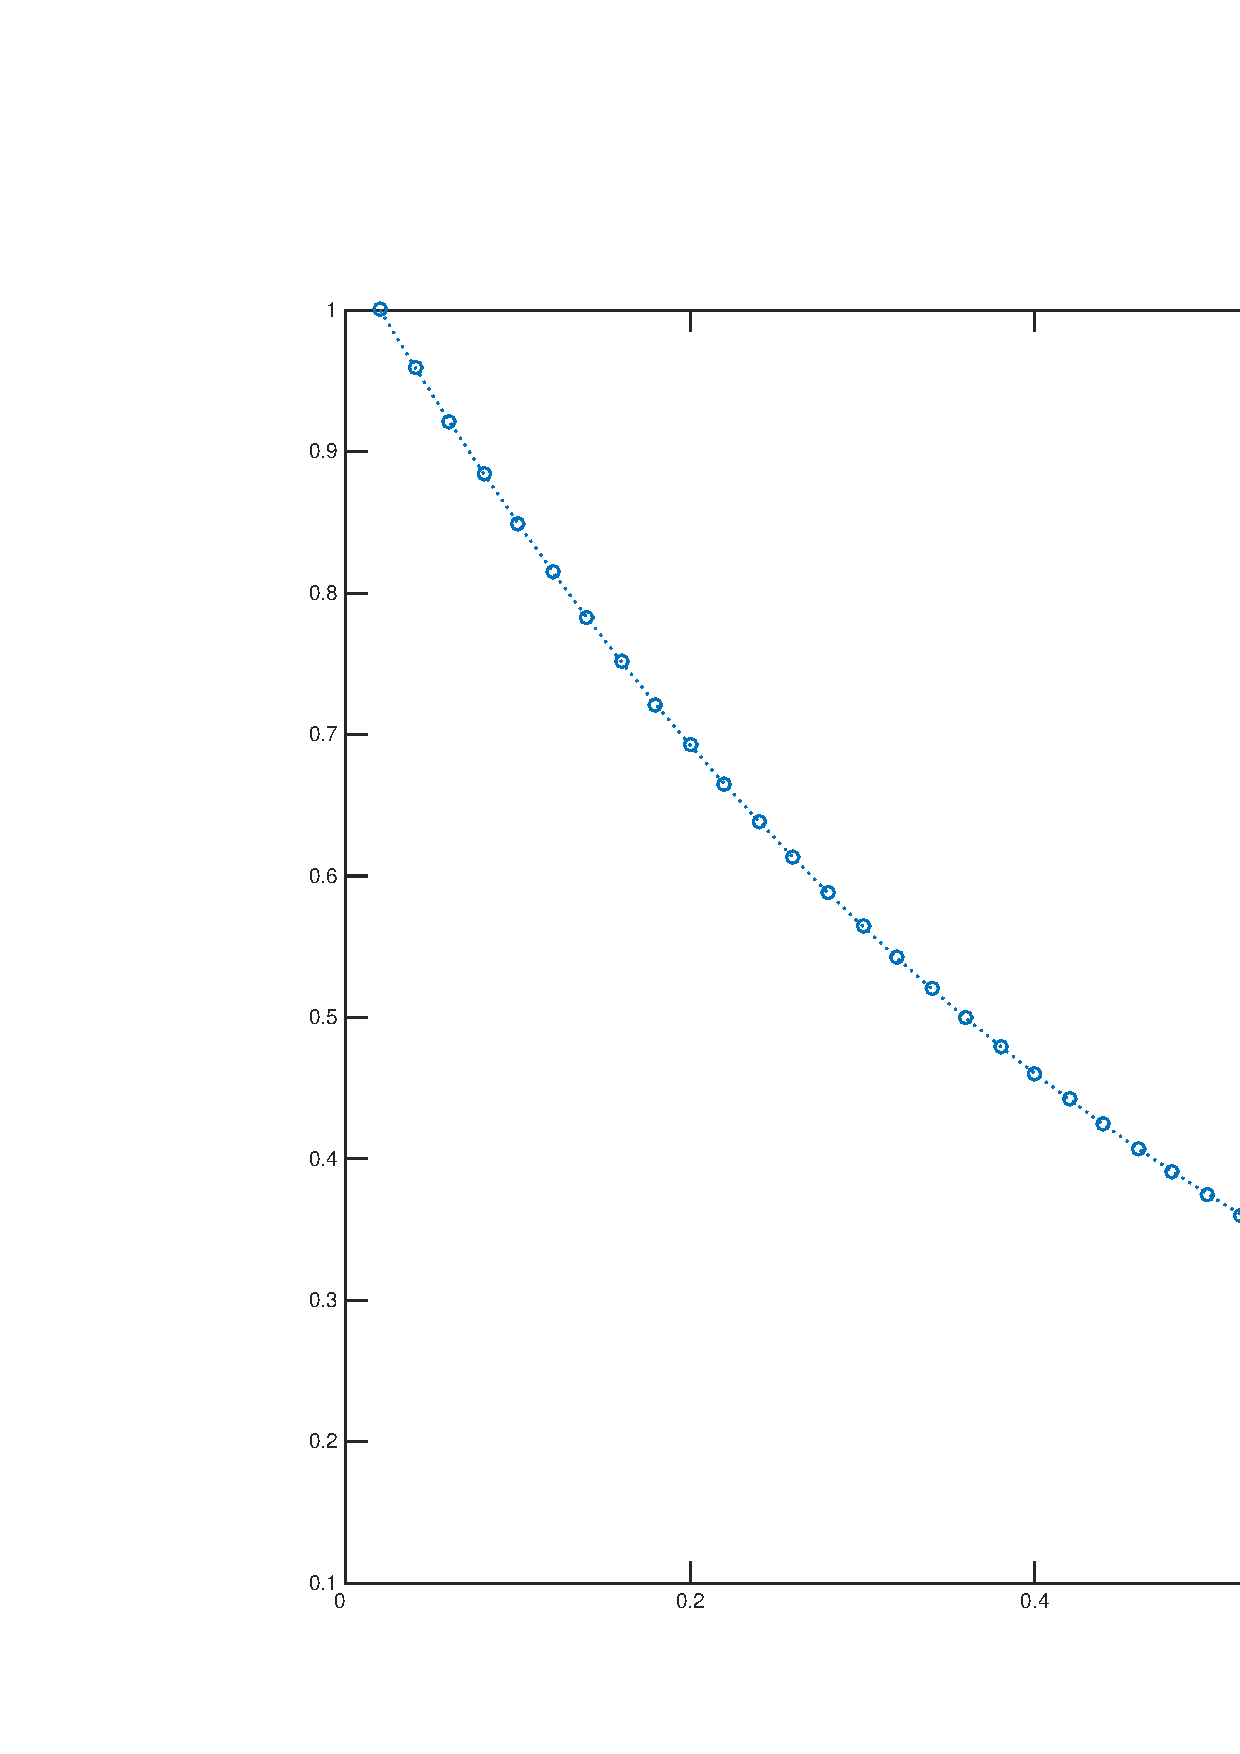
\includegraphics[width=12cm]{1.png}
\end{center}
\[
    \rho(h)=a0.9^{-h/2}\cos(\dfrac{2\pi}4 h+b)
\]

\item[2]
\begin{align*}
	\rho(h)&=c_1z_1^{-h}+\bar c_1\bar z_1^{-h}\\
    &=c_1|z_1|^{-h}e^{-\mathrm{i}\theta h}+\bar c_1|z_1|^{-h}e^{\mathrm{i}\theta h}\\
\tag{$\gamma$ is related to $c_1$, $a$ is a constant}
    &=a|z_1|^{-h}\left(e^{-\mathrm{i}\theta h}+e^{\mathrm{i}\theta h}+e^{\gamma}+e^{-\gamma}\right)\\
\tag{$b$ is a constant}
    &=a|z_1|^{-h}\cos(h\theta+b)
\end{align*}
This is the plot of ACF of Example 3.10, it is exponential decay with sinusoid pattern.\\
\begin{center}
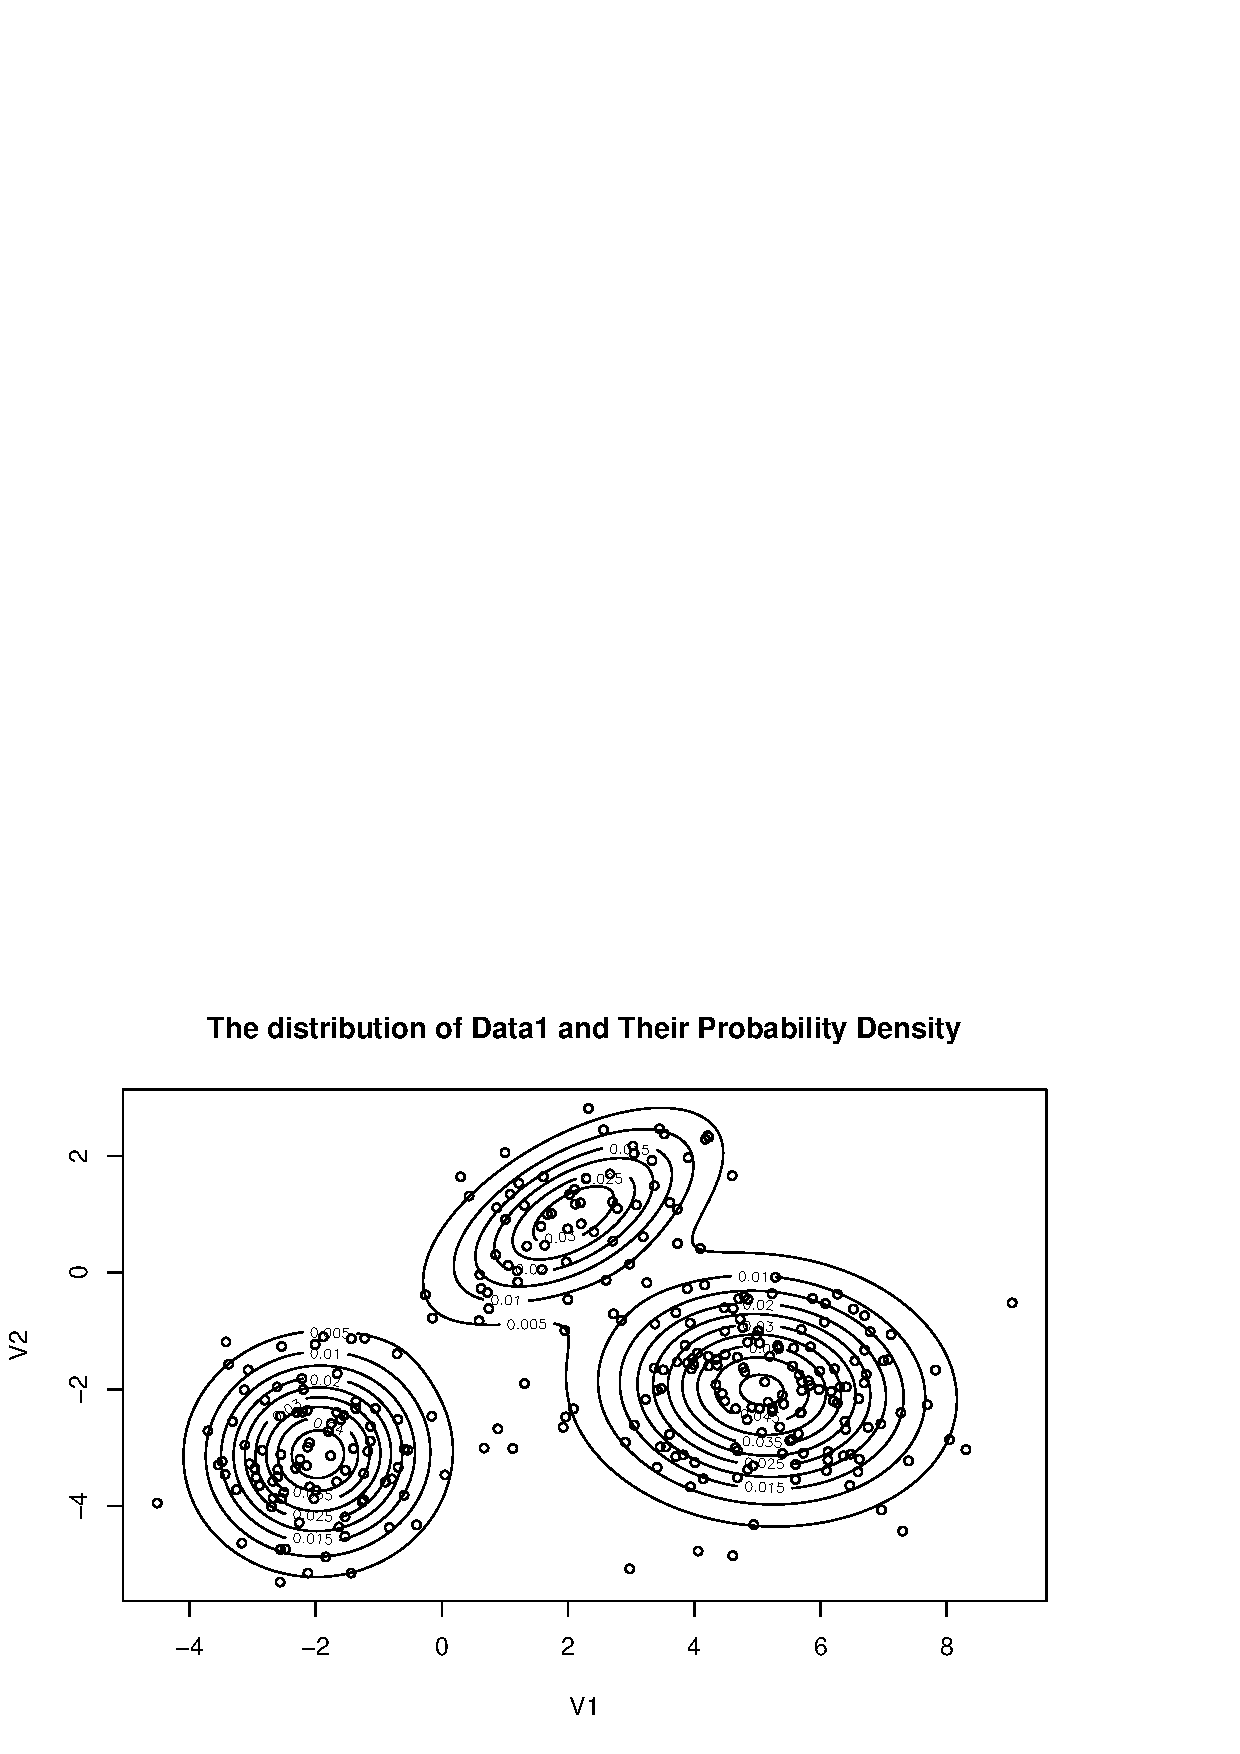
\includegraphics[width=12cm]{2.png}
\end{center}
\end{enumerate}
\end{CJK*}
\end{document}
